% chinthakawk@gmail.com

\documentclass[compress]{beamer} %this is to use copressed header from the
\usepackage{etex}
\usepackage{beamerthemeshadow} %our theme, later you can change it
\usepackage[frenchb]{babel}
\usepackage{fancyhdr} % Required for custom headers
\usepackage[utf8]{inputenc}
\usepackage[lined,boxed]{algorithm2e}
\usepackage[all]{xy}
\usepackage{animate} %need the animate.sty file
\graphicspath{{./Figure/}} 
% editing header
\setbeamertemplate{headline}
{
  \leavevmode%
  \hbox{%
  \begin{beamercolorbox}[wd=.5\paperwidth,ht=2.25ex,dp=1.8ex,leftskip=1em,left]{section in head/foot}%
    \usebeamerfont{subsection in head/foot}\hspace*{5ex}\insertsectionhead
  \end{beamercolorbox}%
  \begin{beamercolorbox}[wd=.5\paperwidth,ht=2.25ex,dp=1.8ex,left,leftskip=1em]{subsection in head/foot}%
    \usebeamerfont{section in head/foot}\insertshorttitle\hspace*{2ex}
  \end{beamercolorbox}}%
  \vskip0pt%
}

% editing footer
\setbeamertemplate{footline}
{
  \leavevmode%
  \hbox{%
  \begin{beamercolorbox}[wd=.5\paperwidth,ht=2.25ex,dp=1ex,right]{author in head/foot}%
    \usebeamerfont{author in head/foot}\insertshortauthor\hspace*{2ex}
  \end{beamercolorbox}%
  \begin{beamercolorbox}[wd=.5\paperwidth,ht=2.25ex,dp=1ex,right]{date in head/foot}%
    \usebeamerfont{date in head/foot}\insertshortdate{}\hspace*{2em}
    \insertframenumber{} / \inserttotalframenumber\hspace*{2ex} 
  \end{beamercolorbox}}%
  \vskip0pt%
}
\definecolor{orange}{rgb}{1,0.5,0}
\definecolor{darkgreen}{rgb}{0,0.5,0}
\definecolor{darkblue}{rgb}{0,0,0.5}

\def\etal{et al.\ }
\def\ie{i.e.\ }
\def\eg{e.g.\ }

%put a wide hat over the argumetn
\newcommand{\lift}[1]{\ensuremath{\widehat{#1}}}

%put a wide hat over the argumetn
%\newcommand{\lifto}[1]{\ensuremath{\check{#1}}}
\newcommand{\lifto}[1]{\ensuremath{\overset{_{_{\circ}}}{#1}}}


% stack vector
\newcommand{\stackv}[1]{\ensuremath{\vet{v}\left( {#1} \right)}}
\newcommand{\ustackv}[1]{\ensuremath{\inv{\vet{v}}\left( {#1} \right)}}

% symmetric stack vector
\newcommand{\stackvs}[1]{\ensuremath{\vet{v}_{\textit{sym}}\left( {#1} \right)}}

% Matrix Lifting: put a wide hat over the argument intended to be a matrix
\newcommand{\mlift}[1]{\ensuremath{\lift{\mat{#1}}}}
\newcommand{\mlifto}[1]{\ensuremath{\lifto{\mat{#1}}}}

% Vector Lifting: put a wide hat over the argument intended to be a matrix
\newcommand{\vlift}[1]{\ensuremath{\lift{\vet{#1}}}}
\newcommand{\vlifto}[1]{\ensuremath{\lifto{\vet{#1}}}}

\newcommand{\bmat}[1]{\ensuremath{\begin{bmatrix} #1 \end{bmatrix}}}
% Vector: print the argument as a vector
\newcommand{\vet}[1]{\ensuremath{\mathbf{#1}}}

% Matrix: print the argument as a matrix
\newcommand{\mat}[1]{\ensuremath{\,\mathtt{#1}\,}}

% Inverse: print a -1 on the top right of the argument 
\newcommand{\inv}[1]{\ensuremath{{#1}^{\text{-}1}}}

% Inverse: print a -1 on the top right of the argument 
\newcommand{\minv}[1]{\ensuremath{\mat{{#1}}^{\text{-}1}}}

% Transpose: print a T on the top right of the argument 
\newcommand{\tra}[1]{\ensuremath{{#1}^{\!\mathsf{T}}}}

% Transpose Matrix: print a T on the top right of the argument intended to be a matrix 
\newcommand{\mtra}[1]{\ensuremath{\tra{\mat{#1}}}}

% Transpose Vector: print a T on the top right of the argument intended to be a vector
\newcommand{\vtra}[1]{\ensuremath{\tra{\vet{#1}}}}

% minus transpose:  print a -T on the top right of the argument
\newcommand{\ment}[1]{\ensuremath{{#1}^{\text{-}\mathsf{T}}}}

% minus transpose matrix:  print a -T on the top right of the argument
\newcommand{\mment}[1]{\ensuremath{{\mat{#1}}^{\text{-}\mathsf{T}}}}

% Cross Matrix:  print the argument in the cross matrix notation
\newcommand{\crmat}[1]{\ensuremath{\left[{#1}\right]_{\times}}}

%enable numbering captions for the images
\setbeamertemplate{caption}[numbered]

%begining of the doc
\begin{document}

 \title{Statistic Criterion for Patch Comparison}  
 %\author{Jia LI}
 %\date{August, 2013} 

 %title page
 \begin{frame}
\titlepage
    \centering
    \begin{minipage}{0.4\textwidth}
    \begin{flushleft} \large
    \emph{Author:}\\
    Dalens Théophile\\
    LI Jia\\
    
    \end{flushleft}
    \end{minipage}
    \begin{minipage}{0.4\textwidth}
    \begin{flushright} \large
    \emph{Course:}\\
    Imagerie Satellitaire
    \end{flushright}
    \end{minipage}\\[3cm]
 \end{frame}
 \section{Introduction}
 \begin{frame}
  \frametitle{Introduction}
	\begin{figure}[h!]
	\centering
	\begin{minipage}{0.7\linewidth}
	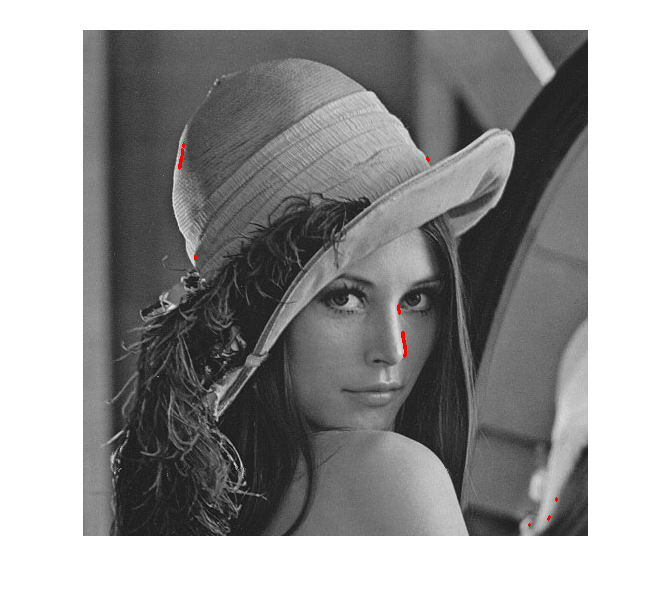
\includegraphics[width=\linewidth]{lena}
	\end{minipage}
	    \caption{Example of application of such techniques}
	\end{figure}
 \end{frame}

 %ToC page
 \begin{frame}
 \scriptsize
 {
 \begin{enumerate}


  \item \textbf{A contrario method}
  \begin{enumerate}
   \item Modeling
   \item Statistic
   \item Approach
   
  \end{enumerate}

  \item Likelihood ratio
  \item Likelihood ratio with learned prior
  \item Comparison
  
 \end{enumerate}

  %\frametitle{Table of contents}
  %\tableofcontents
  
 }
 \end{frame} 
 
 \section{A contrario Method}
 \begin{frame}
  \frametitle{Modeling}
  A patch is considered as a random variable $\mathbb{B}=c_i \mat{B}_i$ a linear combination of reference patches, where $c_i$ are independent random variable following a distribution $h_i$.
	\begin{figure}[h!]
	\centering
	\begin{minipage}{0.4\linewidth}
	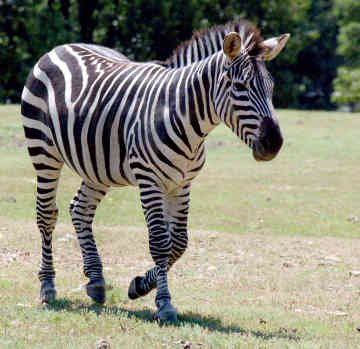
\includegraphics[width=\linewidth]{zebra.jpg}
	  
	\end{minipage}
	\begin{minipage}{0.4\linewidth}
	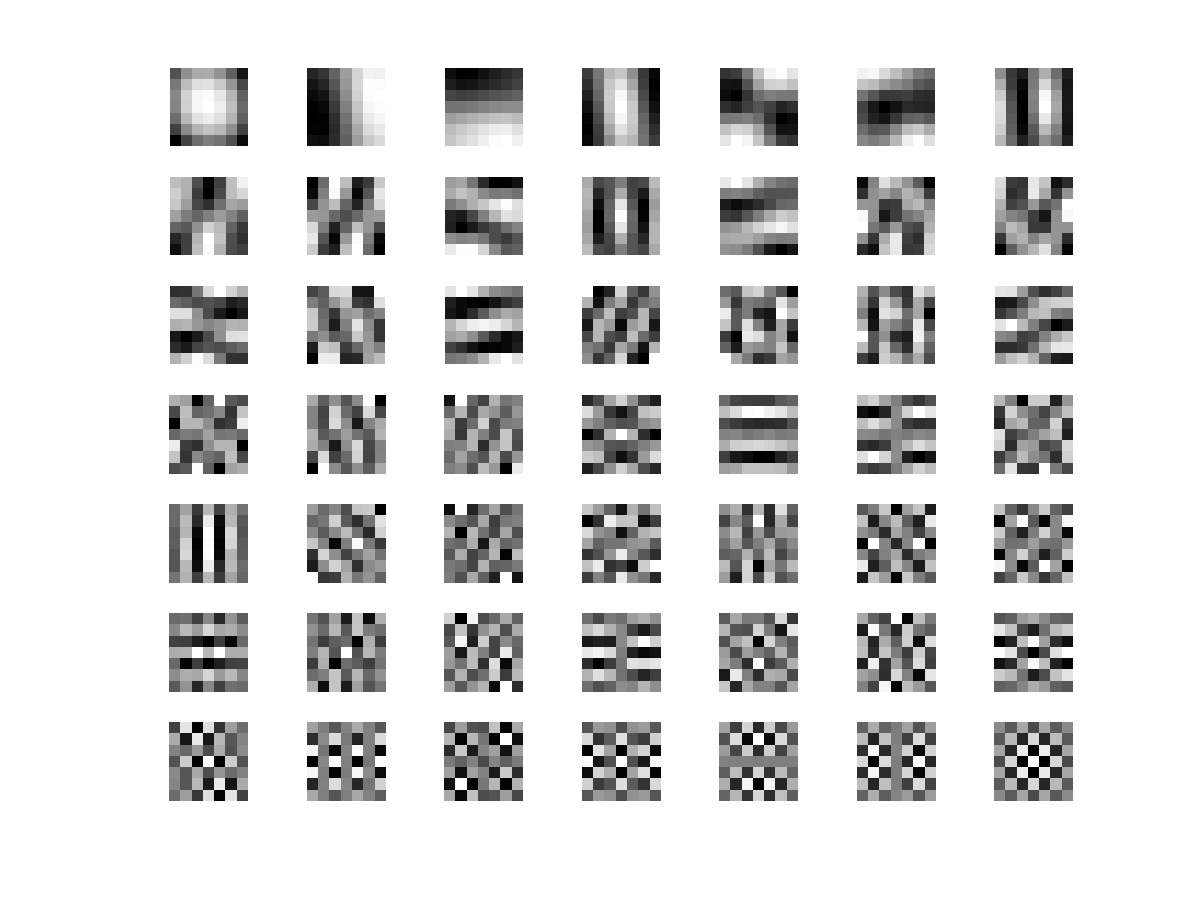
\includegraphics[width=\linewidth]{princomp_zebra.png}
    
	\end{minipage}
	    \caption{Left: A natural image; right: reference patches}
	
	\end{figure}      
 \end{frame}
 \begin{frame}
  \frametitle{Modeling}
  A patch is considered as a random variable $\mathbb{B}=c_i \mat{B}_i$ a linear combination of reference patches, where $c_i$ are independent random variable following a distribution $h_i$.
	\begin{figure}[h!]
	\centering
	\begin{minipage}{0.4\linewidth}
	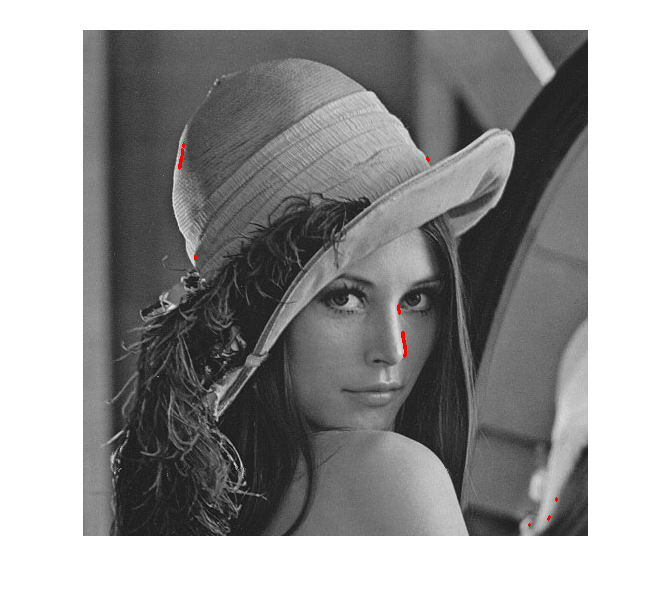
\includegraphics[width=\linewidth]{lena}
	  
	\end{minipage}
	\begin{minipage}{0.4\linewidth}
	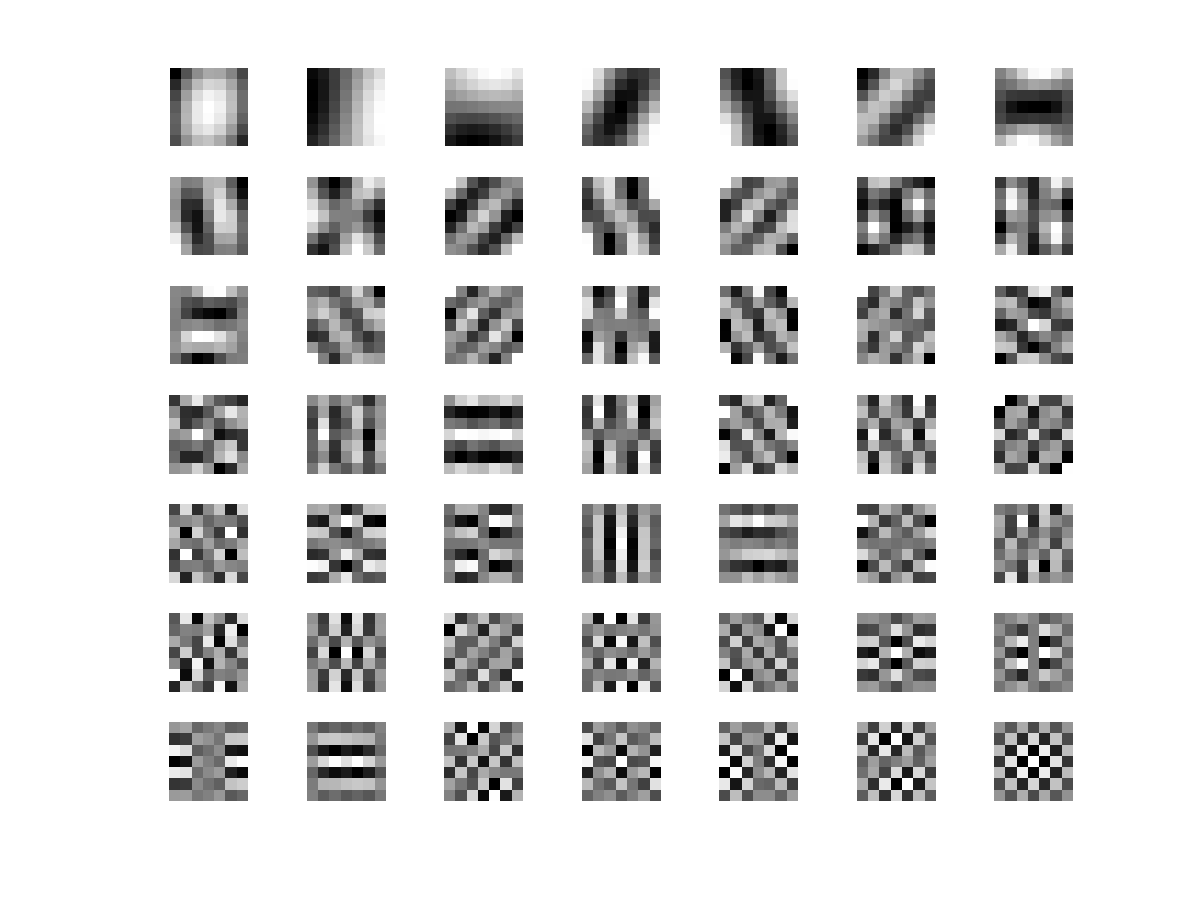
\includegraphics[width=\linewidth]{princomp_lena.png}
    
	\end{minipage}
	    \caption{Left: A natural image; right: reference patches}
	
	\end{figure}      
 \end{frame}
  \begin{frame}
  \frametitle{Modeling}
	\begin{figure}[h!]
	\centering
	\begin{minipage}{0.8\linewidth}
	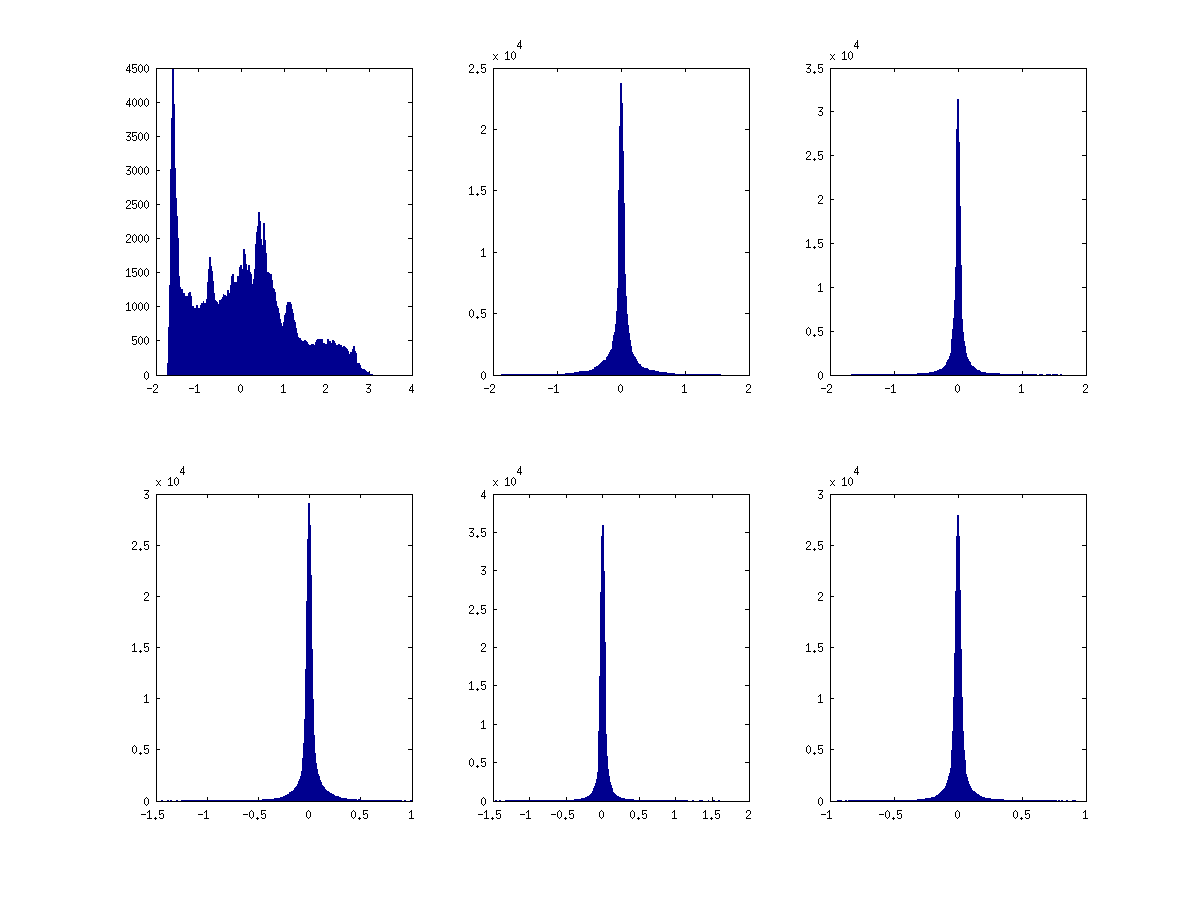
\includegraphics[width=\linewidth]{hist}
	  
	\end{minipage}

	    \caption{Distribution of the firsts components}
	
	\end{figure}      
 \end{frame}
 
 \section{Likelihood ration with learned prior}
 \begin{frame}
 \scriptsize
 {
 \begin{enumerate}


  \item A contrario method
  \item Likelihood ratio
  \item \textbf{Likelihood ratio with learned prior}
  \begin{enumerate}
   \item motivation
   \item approach
   \item result
  \end{enumerate}

  \item Comparison
  
 \end{enumerate}

  %\frametitle{Table of contents}
  %\tableofcontents
  
 }
 \end{frame} 
 
 \begin{frame}
  \frametitle{Approach}
  likelihood ratio :
  \[
  \begin{split}
   P(x_1,x_2 \arrowvert \mathcal{H}_0)&=\int P(x_1 \arrowvert \theta_{12}) P(x_2 \arrowvert \theta_{12}) p(\theta_{12}) d\theta_{12}
  \end{split}
  \]
  
  \[
  \begin{split}
   p(\theta_{12}) d\theta_{12}=\prod_i h_i(c_i)dc_i
  \end{split}
  \]
 \end{frame}


\begin{frame}
\frametitle{Results for different methods}
\begin{figure}
\centering
\begin{minipage}{0.7\linewidth}
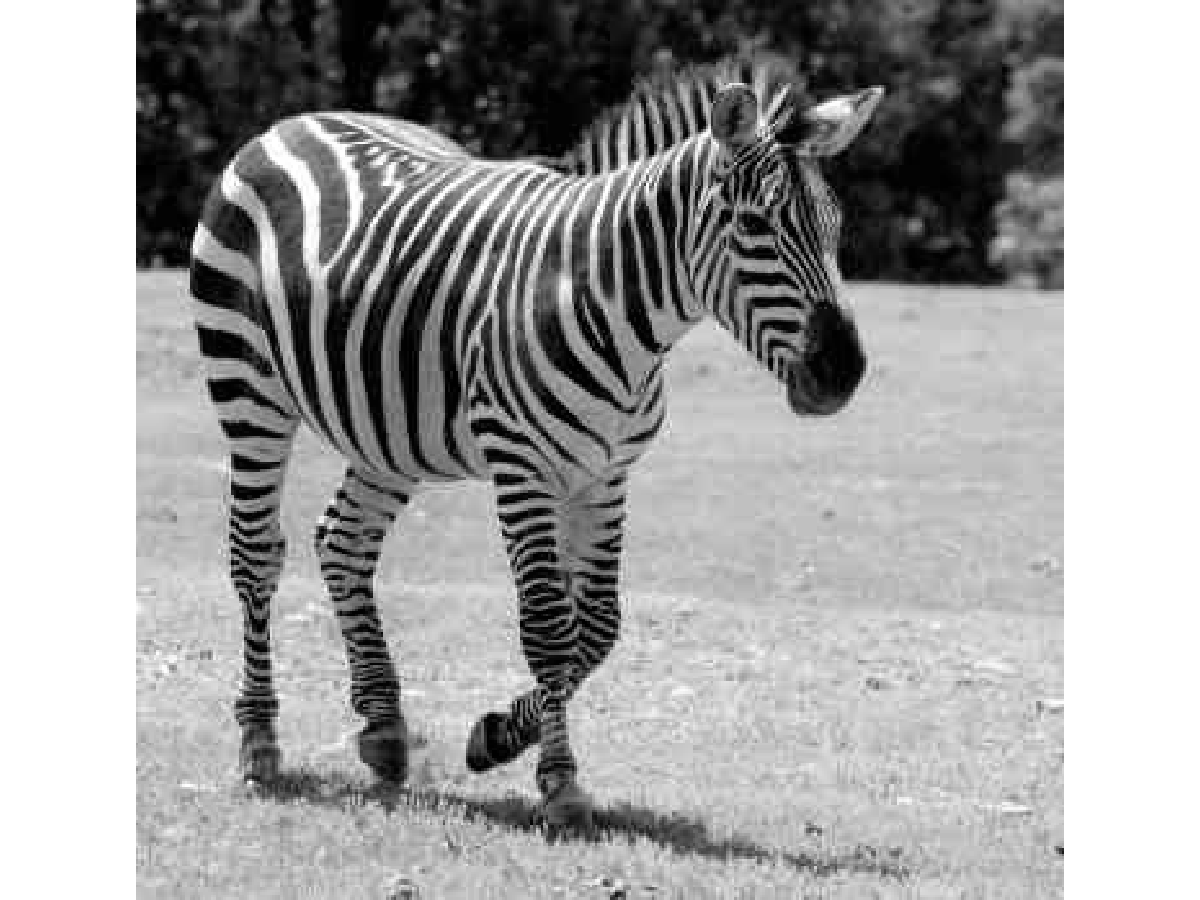
\includegraphics[width=\linewidth]{zebra.png}
\end{minipage}
\begin{minipage}{0.2\linewidth}

\includegraphics[width=\linewidth]{zebra_patch.jpg}
\end{minipage}
\end{figure}
\end{frame}

\begin{frame}
\frametitle{Results for different methods}
\begin{figure}
\centering
\begin{minipage}{0.3\linewidth}
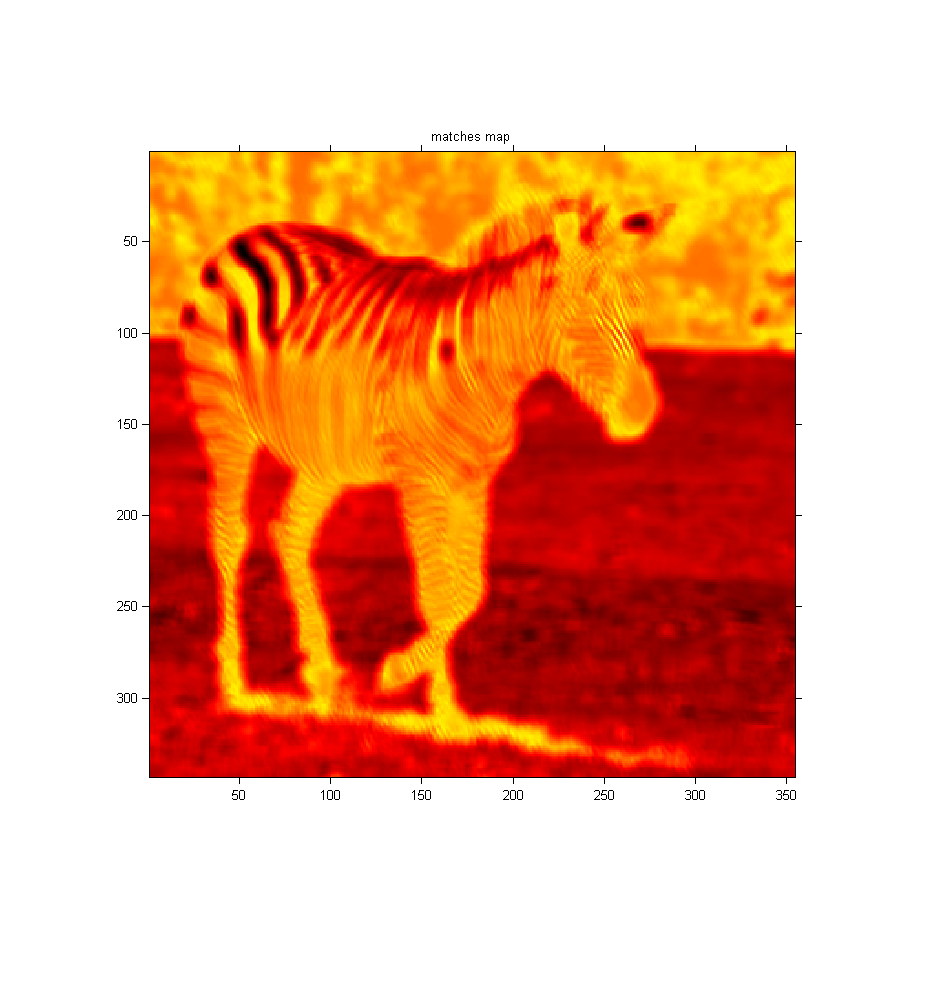
\includegraphics[width=1.3\linewidth]{zebra_heatmap_euclidian.png}
\end{minipage}
\begin{minipage}{0.3\linewidth}
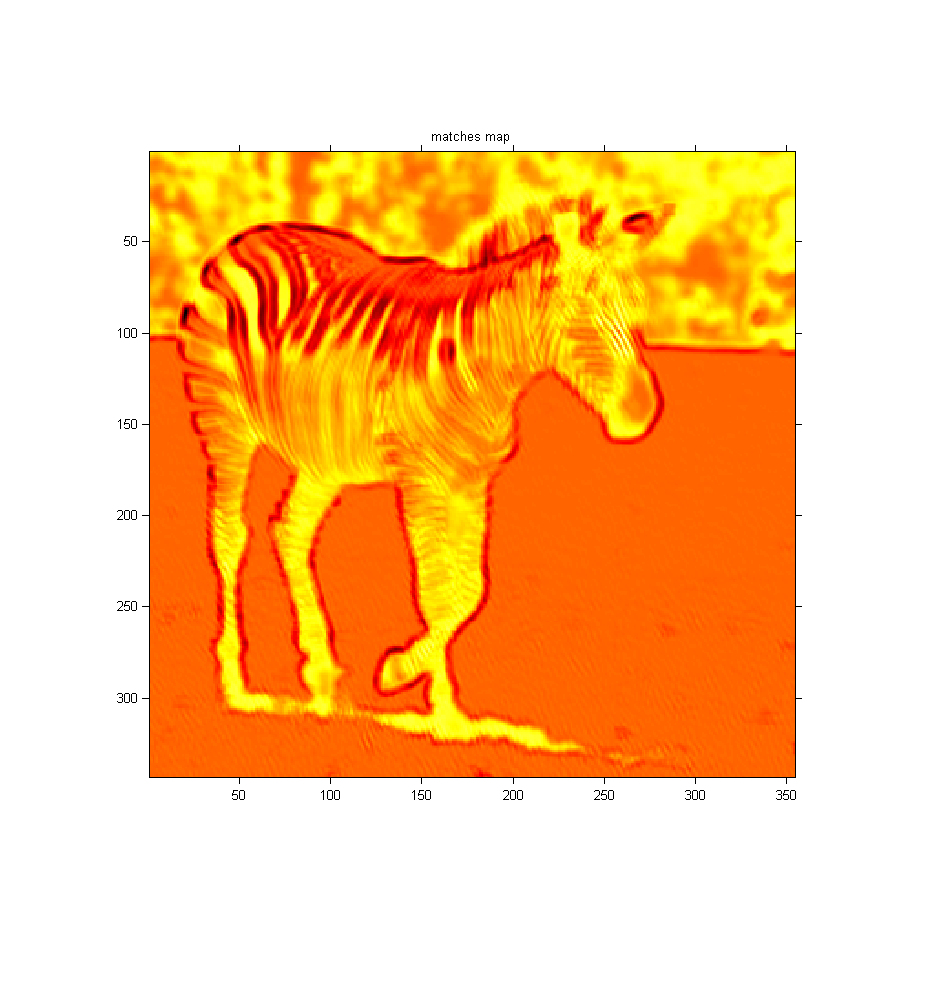
\includegraphics[width=1.3\linewidth]{zebra_heatmap_similarity.png}
\end{minipage}
\begin{minipage}{0.3\linewidth}
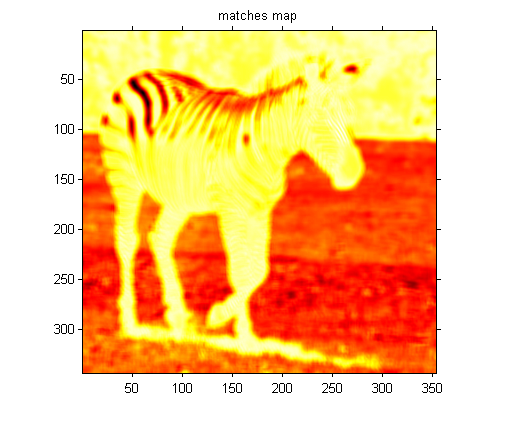
\includegraphics[width=1.3\linewidth]{zebra_heatmap_approx.png}
\end{minipage}
\end{figure}
\end{frame}

\begin{frame}
\frametitle{Results for different methods}
\begin{figure}
\centering
\begin{minipage}{0.3\linewidth}
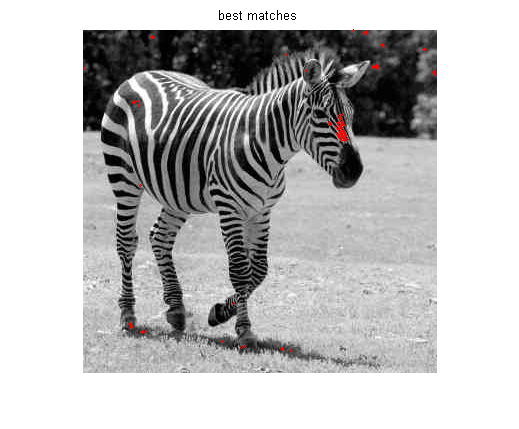
\includegraphics[width=1.3\linewidth]{zebra_best_matches_euclidian.png}
\end{minipage}
\begin{minipage}{0.3\linewidth}
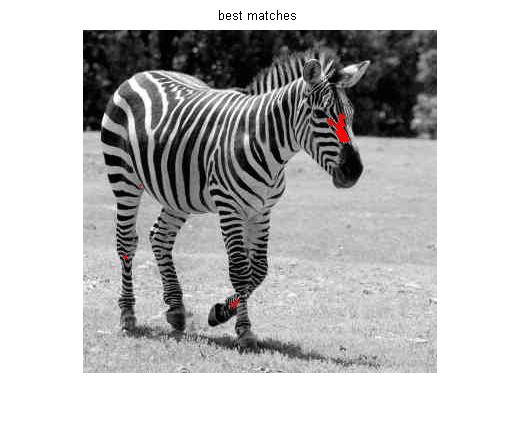
\includegraphics[width=1.3\linewidth]{zebra_best_matches_similarity.png}
\end{minipage}
\begin{minipage}{0.3\linewidth}
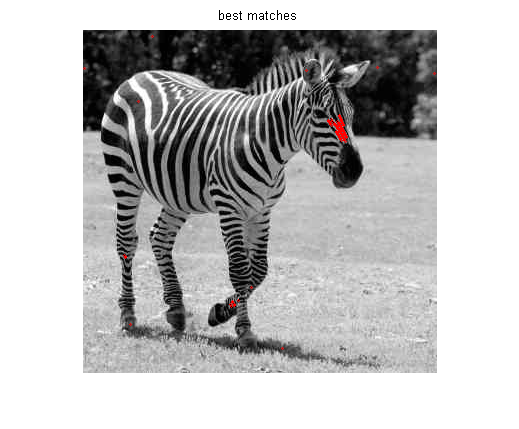
\includegraphics[width=1.3\linewidth]{zebra_best_matches_approx.png}
\end{minipage}
\end{figure}
\end{frame}

\begin{frame}
\frametitle{Likelihood ratio}
The generalized likelihood ratio uses the maximum likelihood estimates for the noise-free patches.
\[
L_G(\mathbf{x_1},\mathbf{x_2})=\frac{\sup_\mathbf{t}p(\mathbf{x_1},\mathbf{x_2};\theta_{12}=\mathbf{t},\mathcal{H}_0)}{\prod_{i=1,2}\sup_\mathbf{t_i}p(\mathbf{x_i};\mathbf{\theta_i}=\mathbf{t_i}}
\]
This comes down to using euclidian distance when the prior is non-informative.
\end{frame}
  
  \begin{frame}
   {\Huge
     \vspace {0.15\textwidth}
     \begin{columns}
       \begin{column}{0.3\textwidth}
       \end{column}
       \begin{column}{0.3\textwidth}
        \text{Thank you!}
       \end{column}
       \begin{column}{0.3\textwidth}
       \end{column}
     \end{columns}
   }
   \vspace {0.025\textwidth}
   \begin{center}
   {\huge Q\&A}
   \end{center}
 \end{frame}
  
\end{document}